%%%%%%%%%%%%%%%%%%%%%%%%%%%%%%%%%%%%%%%%%%%%%%%%%%%%%%%%%%%%%%%%%%%%%%%%%%%%%%%%
\subsection{Συμπεράσματα κεφαλαίου}
\label{subsection:02_02_05:01}

Σε αυτό το κεφάλαιο μάς απασχόλησε η ελάττωση του σφάλματος εκτίμησης στάσης
με αιτία τα ευρήματά μας στο προηγούμενο κεφάλαιο
(ενότητα \ref{subsection:02_01_05:02}). Με δεδομένο τη χρήση του φίλτρου
σωματιδίων για το έργο της παρακολούθησης της στάσης ενός ρομπότ, αναλύσαμε τη
διαθέσιμη βιβλιογραφία γύρω από την ελάττωση του σφάλματος εκτίμησης του, και
προτείναμε δύο επιπρόσθετους τρόπους με τους οποίους είναι δυνατή η επίτευξη
του στόχου. Πιο συγκεκριμένα:

\begin{itemize}
  \item Επικεντρωθήκαμε στο μοντέλο παρατηρήσεων του φίλτρου, και, σκεπτόμενοι
        αναλυτικά, θέσαμε την υπόθεση ότι η επιλογή υποσυνόλων από υποθέσεις
        στάσης του, των οποίων οι αναμενόμενες μετρήσεις από αυτές συμβαδίζουν
        περισσότερο με τις εισερχόμενες στο φίλτρο μετρήσεις του αισθητήρα
        αποστάσεων σε σχέση με άλλες υποθέσεις---η επιλογή αυτών των υποθέσεων
        στάσης ως η εκτίμηση του φίλτρου οφείλει να παράγει χαμηλότερα σφάλματα
        στάσης (ενότητα \ref{subsection:02_02_03:01}). Τα ευρήματά μας
        επιβεβαιώνουν την υπόθεση, αλλά έως ένα κατώφλι πληθικότητας αυτών των
        υποσυνόλων: στο όριο, η μοναδική υπόθεση στάσης που εμφανίζει τη
        μεγαλύτερη πιθανότητα παρατήρησης των μετρήσεων από αυτήν εμφανίζει
        μεγαλύτερα σφάλματα στάσης από ότι η συλλογική εκτίμηση του φίλτρου.
        Βάσει αυτού του ευρήματος συμπεράναμε ότι το φίλτρο σωματιδίων δεν
        αποτελεί άθροισμα υποθέσεων, αλλά μία κατακερματισμένη μορφή εκτίμησης.
  \item Ερευνήσαμε και ζητήσαμε να ελέγξουμε την ευστάθεια της υπόθεσης ότι
        το αποτέλεσμα της εφαρμογής του μετασχηματισμού της ευθυγράμμισης
        μετρήσεων δισδιάστατου αισθητήρα lidar με σαρώσεις χάρτη από την
        παραγώμενη εκτίμηση του φίλτρου στην ίδια την εκτίμηση του εμφανίζει
        χαμηλότερα σφάλματα εκτίμησης στάσης σε σχέση με την αρχική εκτίμηση
        (ενότητα \ref{subsection:02_02_03:02}). Με βάση τη διαμόρφωση της
        πειραματικής διαδικασίας, τα ευρήματα αποδεικνύουν ότι η εφαρμογή της
        διαδικασίας ευθυγράμμισης έχει σημαντικά οφέλη στην ελάττωση του
        σφάλματος εκτίμησης.
  \item Παρακινούμενοι από ελλείψεις και μεινοκτήματα μεθόδων της τρέχουσας
        βιβλιογραφίας προτείναμε έναν τρόπο ανάδρασης του αποτελέσματος της
        ευθυγράμμισης μετρήσεων με σαρώσεις χάρτη στον πληθυσμό του φίλτρου
        σωματιδίων (ενότητα \ref{subsection:02_02_03:03}): δεδομένων ότι το
        αποτέλεσμα της ευθυγράμμισης (α) είναι πιο ακριβές από την εκτίμηση του
        φίλτρου και (β) είναι άγνωστο στο ίδιο το φίλτρο, σχεδιάσαμε έναν
        μηχανισμό ανάδρασης που (i) προκαλεί πιο γρήγορη σύγκλιση και
        χαμηλότερα σφάλματα εκτίμησης σε σχέση με έναν μηχανισμό ανάδρασης της
        βιβλιογραφίας, (ii) προκαλεί την αποφυγή απόκλισης του φίλτρου σε σχέση
        με έναν δεύτερο μηχανισμό ανάδρασης της βιβλιογραφίας, και (iii)
        εμφανίζει χαμηλότερα σφάλματα στάσης σε σχέση με το φίλτρο σε κατάσταση
        ανοιχτού βρόχου.
\end{itemize}

Στο σχήμα \ref{fig:02_02_05:01} απεικονίζονται συνοπτικά οι συμβολές του
παρόντος κεφαλαίου στη μεθοδολογία ελάττωσης του σφάλματος εκτίμησης φίλτρου
σωματιδίων με χρήση αισθητήρων απόστασης τύπου 2D lidar.

\begin{figure}
  \hspace{-1.5cm}
  % GNUPLOT: LaTeX picture with Postscript
\begingroup
  \makeatletter
  \providecommand\color[2][]{%
    \GenericError{(gnuplot) \space\space\space\@spaces}{%
      Package color not loaded in conjunction with
      terminal option `colourtext'%
    }{See the gnuplot documentation for explanation.%
    }{Either use 'blacktext' in gnuplot or load the package
      color.sty in LaTeX.}%
    \renewcommand\color[2][]{}%
  }%
  \providecommand\includegraphics[2][]{%
    \GenericError{(gnuplot) \space\space\space\@spaces}{%
      Package graphicx or graphics not loaded%
    }{See the gnuplot documentation for explanation.%
    }{The gnuplot epslatex terminal needs graphicx.sty or graphics.sty.}%
    \renewcommand\includegraphics[2][]{}%
  }%
  \providecommand\rotatebox[2]{#2}%
  \@ifundefined{ifGPcolor}{%
    \newif\ifGPcolor
    \GPcolorfalse
  }{}%
  \@ifundefined{ifGPblacktext}{%
    \newif\ifGPblacktext
    \GPblacktexttrue
  }{}%
  % define a \g@addto@macro without @ in the name:
  \let\gplgaddtomacro\g@addto@macro
  % define empty templates for all commands taking text:
  \gdef\gplfronttext{}%
  \makeatother
  \ifGPblacktext
    % no textcolor at all
    \def\colorrgb#1{}%
    \def\colorgray#1{}%
  \else
    % gray or color?
    \ifGPcolor
      \def\colorrgb#1{\color[rgb]{#1}}%
      \def\colorgray#1{\color[gray]{#1}}%
      \expandafter\def\csname LTw\endcsname{\color{white}}%
      \expandafter\def\csname LTb\endcsname{\color{black}}%
      \expandafter\def\csname LTa\endcsname{\color{black}}%
      \expandafter\def\csname LT0\endcsname{\color[rgb]{1,0,0}}%
      \expandafter\def\csname LT1\endcsname{\color[rgb]{0,1,0}}%
      \expandafter\def\csname LT2\endcsname{\color[rgb]{0,0,1}}%
      \expandafter\def\csname LT3\endcsname{\color[rgb]{1,0,1}}%
      \expandafter\def\csname LT4\endcsname{\color[rgb]{0,1,1}}%
      \expandafter\def\csname LT5\endcsname{\color[rgb]{1,1,0}}%
      \expandafter\def\csname LT6\endcsname{\color[rgb]{0,0,0}}%
      \expandafter\def\csname LT7\endcsname{\color[rgb]{1,0.3,0}}%
      \expandafter\def\csname LT8\endcsname{\color[rgb]{0.5,0.5,0.5}}%
    \else
      % gray
      \def\colorrgb#1{\color{black}}%
      \def\colorgray#1{\color[gray]{#1}}%
      \expandafter\def\csname LTw\endcsname{\color{white}}%
      \expandafter\def\csname LTb\endcsname{\color{black}}%
      \expandafter\def\csname LTa\endcsname{\color{black}}%
      \expandafter\def\csname LT0\endcsname{\color{black}}%
      \expandafter\def\csname LT1\endcsname{\color{black}}%
      \expandafter\def\csname LT2\endcsname{\color{black}}%
      \expandafter\def\csname LT3\endcsname{\color{black}}%
      \expandafter\def\csname LT4\endcsname{\color{black}}%
      \expandafter\def\csname LT5\endcsname{\color{black}}%
      \expandafter\def\csname LT6\endcsname{\color{black}}%
      \expandafter\def\csname LT7\endcsname{\color{black}}%
      \expandafter\def\csname LT8\endcsname{\color{black}}%
    \fi
  \fi
  \setlength{\unitlength}{0.0500bp}%
  \begin{picture}(10000.00,4000.00)%
    \gplgaddtomacro\gplfronttext{%
      \colorrgb{0.00,0.00,0.00}%
      \put(1168,440){\makebox(0,0)[r]{\strut{}$0.005$}}%
      \colorrgb{0.00,0.00,0.00}%
      \put(1168,1526){\makebox(0,0)[r]{\strut{}$0.010$}}%
      \colorrgb{0.00,0.00,0.00}%
      \put(1168,2613){\makebox(0,0)[r]{\strut{}$0.015$}}%
      \colorrgb{0.00,0.00,0.00}%
      \put(1300,220){\makebox(0,0){\strut{}$200$}}%
      \colorrgb{0.00,0.00,0.00}%
      \put(2091,220){\makebox(0,0){\strut{}$600$}}%
      \colorrgb{0.00,0.00,0.00}%
      \put(2882,220){\makebox(0,0){\strut{}$1000$}}%
      \colorrgb{0.00,0.00,0.00}%
      \put(5000,4600){\makebox(0,0){\strut{}Μέσο σφάλμα εκτίμησης σε $N = 100$ διαδρομές ανά εκτιμώμενη στάση}}%
      \colorrgb{0.00,0.00,0.00}%
      \put(5100,-510){\makebox(0,0){\strut{}Αριθμός εκτιμήσεων στάσης στο χρόνο}}%
      \definecolor{gr}{RGB}{161,214,107}
      \definecolor{pi}{RGB}{232,163,201}
      \definecolor{k}{RGB}{0,0,0}
      \definecolor{sm}{RGB}{227,74,51}
      \put(2110,4229){\makebox(0,0){\strut{}{\color{k}{\rule[0.6mm]{0.5cm}{0.5mm}}} MCL}}
      \put(2200,4000){\makebox(0,0){\strut{}{\color{gr}{\rule[0.6mm]{0.5cm}{0.5mm}}} $\%$MCL}}
      \put(1900,4000){\makebox(0,0){\strut{}{\color{pi}{\rule[0.6mm]{0.25cm}{0.5mm}}}}}

      \put(4700,4229){\makebox(0,0){\strut{}{\color{k}{\rule[0.6mm]{0.5cm}{0.5mm}}} MCL}}
      \put(5100,4000){\makebox(0,0){\strut{}{\color{sm}{\rule[0.6mm]{0.5cm}{0.5mm}}} MCL $\circ$ smsm}}

      \put(7460,4229){\makebox(0,0){\strut{}{\color{k}{\hdashrule[0.6mm]{0.60cm}{0.5mm}{0.5mm}}} MCL}}
      \put(8100,4000){\makebox(0,0){\strut{}{\color{k}{\rule[0.6mm]{0.5cm}{0.5mm}}} MCL $\circ$ smsm $\circ$ $\circlearrowleft$}}

      \put(2210,-100){\makebox(0,0){\strut{} CORRIDOR}}
      \put(5100,-100){\makebox(0,0){\strut{} WAREHOUSE}}
      \put(7990,-100){\makebox(0,0){\strut{} WAREHOUSE}}
    }%
    \gplgaddtomacro\gplfronttext{%
    }%
    \gplgaddtomacro\gplfronttext{%
      \colorrgb{0.00,0.00,0.00}%
      \put(4053,440){\makebox(0,0)[r]{\strut{}$0$}}%
      \colorrgb{0.00,0.00,0.00}%
      \put(4053,1092){\makebox(0,0)[r]{\strut{}$0.02$}}%
      \colorrgb{0.00,0.00,0.00}%
      \put(4053,1744){\makebox(0,0)[r]{\strut{}$0.04$}}%
      \colorrgb{0.00,0.00,0.00}%
      \put(4053,2395){\makebox(0,0)[r]{\strut{}$0.06$}}%
      \colorrgb{0.00,0.00,0.00}%
      \put(4053,3047){\makebox(0,0)[r]{\strut{}$0.08$}}%
      \colorrgb{0.00,0.00,0.00}%
      \put(4053,3699){\makebox(0,0)[r]{\strut{}$0.10$}}%
      \colorrgb{0.00,0.00,0.00}%
      \put(4185,220){\makebox(0,0){\strut{}$0$}}%
      \colorrgb{0.00,0.00,0.00}%
      \put(4734,220){\makebox(0,0){\strut{}$100$}}%
      \colorrgb{0.00,0.00,0.00}%
      \put(5284,220){\makebox(0,0){\strut{}$200$}}%
      \colorrgb{0.00,0.00,0.00}%
      \put(5833,220){\makebox(0,0){\strut{}$300$}}%
    }%
    \gplgaddtomacro\gplfronttext{%
      \colorrgb{0.00,0.00,0.00}%
      \put(6939,440){\makebox(0,0)[r]{\strut{}$0$}}%
      \colorrgb{0.00,0.00,0.00}%
      \put(6939,1092){\makebox(0,0)[r]{\strut{}$0.02$}}%
      \colorrgb{0.00,0.00,0.00}%
      \put(6939,1744){\makebox(0,0)[r]{\strut{}$0.04$}}%
      \colorrgb{0.00,0.00,0.00}%
      \put(6939,2395){\makebox(0,0)[r]{\strut{}$0.06$}}%
      \colorrgb{0.00,0.00,0.00}%
      \put(6939,3047){\makebox(0,0)[r]{\strut{}$0.08$}}%
      \colorrgb{0.00,0.00,0.00}%
      \put(6939,3699){\makebox(0,0)[r]{\strut{}$0.10$}}%
      \colorrgb{0.00,0.00,0.00}%
      \put(7071,220){\makebox(0,0){\strut{}$0$}}%
      \colorrgb{0.00,0.00,0.00}%
      \put(7620,220){\makebox(0,0){\strut{}$100$}}%
      \colorrgb{0.00,0.00,0.00}%
      \put(8170,220){\makebox(0,0){\strut{}$200$}}%
      \colorrgb{0.00,0.00,0.00}%
      \put(8719,220){\makebox(0,0){\strut{}$300$}}%
    }%
    \put(0,0){\includegraphics{./figures/parts/02/chapters/02/sections/05/h_123}}%
    \gplfronttext
  \end{picture}%
\endgroup

  \vspace{1cm}
  \caption{\small Η συμβολή των μεθόδων που παρουσιάστηκαν στο παρόν κεφάλαιο
           ως προς το μέσο σφάλμα εκτίμησης ανά στάση στα διενεργηθέντα
           πειράματα. Αριστερά: με μαύρο χρώμα το αποτέλεσμα του MCL και με άλλα
           χρώματα το αποτέλεσμα της επιλογής υποσυνόλων σωματιδίων στο
           περιβάλλον CORRIDOR. Μέση: με μαύρο χρώμα το αποτέλεσμα του MCL και
           με κόκκινο το αποτέλεσμα της ευθυγράμμισης μετρήσεων δισδιάστατου
           αισθητήρα lidar με σαρώσεις χάρτη (smsm). Δεξιά: με διακεκομμένη
           γραμμή το αποτέλεσμα του MCL και με συνεχή το αποτέλεσμα του ολικού
           συστήματος (σχήμα \ref{fig:overall_system}) μετά την ανατροφοδότηση
           του αποτελέσματος της ευθυγράμμισης μετρήσεων με σαρώσεις χάρτη
           στον πληθυσμό του φίλτρου μέσω της προτεινόμενης μεθόδου
           ανατροφοδότησης}
  \label{fig:02_02_05:01}
\end{figure}


%%%%%%%%%%%%%%%%%%%%%%%%%%%%%%%%%%%%%%%%%%%%%%%%%%%%%%%%%%%%%%%%%%%%%%%%%%%%%%%%
\subsection{Αιτίες περαιτέρω έρευνας}
\label{subsection:02_02_05:02}

Κατά τη διάρκεια διεξαγωγής της υλοποίησης του σύνθετου συστήματος περάσαμε
από το στάδιο ενσωμάτωσης του αλγορίθμου ευθυγράμμισης των δισδιάστατων
μετρήσεων του αισθητήρα lidar με τις σαρώσεις χάρτη, ήτοι του PLICP. Προτού
τον ενσωματώσουμε οριστικά στο σύνθετο σύστημα τον υποβάλαμε σε μία σειρά από
δοκιμές ώστε να επαληθεύσουμε τη ορθότητά των αποτελεσμάτων που εμφανίζονται
στη βιβλιογραφία και αφορούν σε αυτόν, αλλά στα συμφραζόμενα της έρευνας μας.
Κατά τη διάρκεια αυτών των δοκιμών καταλήξαμε σε μία σειρά από συμπεράσματα,
τα οποία παρουσιάζουμε παρακάτω. ??

Ένα κύριο πρόβλημα---αν όχι το κυριότερο---στο οποίο πρέπει να δοθεί προσοχή
είναι η πρακτική της εύρεσης αντιστοιχίσεων ανάμεσα στις ακτίνες των εισόδων
του PLICP. Αυτό αφορά σε όλες τις προσεγγίσεις ευθυγραμμίσεων σαρώσεων με
σαρώσεις (πραγματικών μετρήσεων με πραγματικές μετρήσεις ή με εικονικές
μετρήσεις από χάρτη) όπως η μέθοδος ICP και η πληθώρα των παραλλαγών της. Το
πρόβλημα εδώ είναι ότι, δεδομένου του θορύβου του αισθητήρα μέτρησης και των
αποκλίσεων μεταξύ του χάρτη και περιβάλλοντος, η δημιουργία αντιστοιχιών μπορεί
να οδηγήσει σε ανακριβή αποτελέσματα ή συνολικά σε αποκλίνοντα αποτελέσματα.
Στην πράξη, όσον αφορά τις μεθόδους που λειτουργούν απευθείας στο χώρο των
μετρήσεων, το φιλτράρισμα των ακραίων τιμών πραγματοποιείται μέσω διαδικασιών
που εξαρτώνται από την εκπλήρωση των υποθέσεων και την ακριβή ρύθμιση εξωτερικά
παρεχόμενων παραμέτρων. Αυτές οι παράμετροι περιλαμβάνουν, για παράδειγμα, μια
εκτίμηση της τυπικής απόκλισης του κανονικά κατανεμημένου θορύβου μηδενικής
μέσης τιμής που επιδρά στις μετρήσεις ενός αισθητήρα αποστάσεων--όταν οι
μετρήσεις του αισθητήρα μπορεί στην πραγματικότητα να είναι μεροληπτικές
(biased), ή να μην ικανοποιούν την υπόθεση της κανονικής κατανομής του θορύβου
τους \cite{Cooper2018a}---, ή μια εκτίμηση του ποσοστού των ακραίων τιμών στις
εισόδους τους.

Αυτό μας οδηγεί σε ένα άλλο κρίσιμο σημείο, δηλαδή το ζήτημα της
παραμετροποίησης. Η επίδοση της πλειονότητας των μεθόδων ευθυγράμμισης σάρωσης
(σε χάρτη) - όχι όχι μόνο εκείνων που βασίζονται στην ICP-- στηρίζεται στον
ακριβή συντονισμό των παραμέτρων που διέπουν τις εσωτερικές τους διαδικασίες.
Γενικά, θεωρείται ορθά ότι οι εν λόγω παράμετροι πρέπει να συντονίζονται για
ένα συγκεκριμένο περιβάλλον και για συγκεκριμένο θόρυβο επίπεδα θορύβου, αλλά
στην πραγματικότητα, ελλείψει αυτόματης on-line ρύθμισης των παραμέτρων,
διαφορετικές παραμετροποιήσεις μπορεί να οδηγήσουν σε ασταθή ή μη διαισθητικά
αποτελέσματα- και το αποτέλεσμα αυτό μπορεί να εμφανιστεί ακόμη και για την
ίδια πόζα στο ίδιο περιβάλλον.  Ας αποσαφηνίσουμε αυτή την ιδιότητα με ένα απλό
αλλά χαρακτηριστικό παράδειγμα.

Ας υποθέσουμε ένα αρκετά συνηθισμένο σενάριο: ο συνολικός εντοπισμός πρέπει να πραγματοποιηθεί σε
περιβάλλον από ένα ρομπότ εξοπλισμένο μόνο με έναν αισθητήρα 2D LIDAR. Ας υποθέσουμε επίσης
ότι για λόγους γενικότητας, δηλαδή για χρήση σε άγνωστα, διαφορετικά και ανομοιογενή
περιβάλλοντα, η υποκείμενη μέθοδος εντοπισμού απαιτείται να είναι ισχυρή και
συνεπώς να αποφεύγεται η χρήση χαρακτηριστικών. Ένας τρόπος επίλυσης αυτού του προβλήματος είναι η διασπορά ενός
πεπερασμένου αριθμού υποθέσεων πόζας στον μη κατειλημμένο χώρο που περιορίζεται εντός του
όρια του χάρτη και να εκτελείται μια αντιστοίχιση σάρωσης-προς-χάρτη-σάρωσης μεταξύ του εύρους
σάρωσης που λαμβάνεται από τον φυσικό αισθητήρα LIDAR και της σάρωσης χάρτη που προκύπτει από κάθε
υπόθεση. Μια φυσική επιλογή θα ήταν να χρησιμοποιηθεί το ICP ή μια από τις παραλλαγές του, όπως
έχουν αποδείξει την αποτελεσματικότητα και την ευρωστία τους σε διάφορα πλαίσια
\cite{paid_original}\cite{plicp}\cite{ICP}- όλα ασχολούνται με αντιστοιχίες και
απαιτούν ρυθμιζόμενες παραμέτρους, οι οποίες αφορούν λειτουργίες που περιλαμβάνουν, αλλά όχι
που αφορούν, μεταξύ άλλων, την καθιέρωση αντιστοιχιών με φιλτράρισμα των ακραίων τιμών. Το αποτέλεσμα της
αυτής της μεθόδου συνολικού εντοπισμού θα είναι η πόζα για την οποία η ICP αναφέρει
το χαμηλότερο σφάλμα αντιστοίχισης (εξ. \ref{eq:min_err_icp}).

%\begin{figure}\centering
  %\definecolor{r}{RGB}{255 0 0}
\definecolor{g}{RGB}{0 155 0}
% GNUPLOT: LaTeX picture with Postscript
\begingroup
  \makeatletter
  \providecommand\color[2][]{%
    \GenericError{(gnuplot) \space\space\space\@spaces}{%
      Package color not loaded in conjunction with
      terminal option `colourtext'%
    }{See the gnuplot documentation for explanation.%
    }{Either use 'blacktext' in gnuplot or load the package
      color.sty in LaTeX.}%
    \renewcommand\color[2][]{}%
  }%
  \providecommand\includegraphics[2][]{%
    \GenericError{(gnuplot) \space\space\space\@spaces}{%
      Package graphicx or graphics not loaded%
    }{See the gnuplot documentation for explanation.%
    }{The gnuplot epslatex terminal needs graphicx.sty or graphics.sty.}%
    \renewcommand\includegraphics[2][]{}%
  }%
  \providecommand\rotatebox[2]{#2}%
  \@ifundefined{ifGPcolor}{%
    \newif\ifGPcolor
    \GPcolorfalse
  }{}%
  \@ifundefined{ifGPblacktext}{%
    \newif\ifGPblacktext
    \GPblacktexttrue
  }{}%
  % define a \g@addto@macro without @ in the name:
  \let\gplgaddtomacro\g@addto@macro
  % define empty templates for all commands taking text:
  \gdef\gplfronttext{}%
  \gdef\gplfronttext{}%
  \makeatother
  \ifGPblacktext
    % no textcolor at all
    \def\colorrgb#1{}%
    \def\colorgray#1{}%
  \else
    % gray or color?
    \ifGPcolor
      \def\colorrgb#1{\color[rgb]{#1}}%
      \def\colorgray#1{\color[gray]{#1}}%
      \expandafter\def\csname LTw\endcsname{\color{white}}%
      \expandafter\def\csname LTb\endcsname{\color{black}}%
      \expandafter\def\csname LTa\endcsname{\color{black}}%
      \expandafter\def\csname LT0\endcsname{\color[rgb]{1,0,0}}%
      \expandafter\def\csname LT1\endcsname{\color[rgb]{0,1,0}}%
      \expandafter\def\csname LT2\endcsname{\color[rgb]{0,0,1}}%
      \expandafter\def\csname LT3\endcsname{\color[rgb]{1,0,1}}%
      \expandafter\def\csname LT4\endcsname{\color[rgb]{0,1,1}}%
      \expandafter\def\csname LT5\endcsname{\color[rgb]{1,1,0}}%
      \expandafter\def\csname LT6\endcsname{\color[rgb]{0,0,0}}%
      \expandafter\def\csname LT7\endcsname{\color[rgb]{1,0.3,0}}%
      \expandafter\def\csname LT8\endcsname{\color[rgb]{0.5,0.5,0.5}}%
    \else
      % gray
      \def\colorrgb#1{\color{black}}%
      \def\colorgray#1{\color[gray]{#1}}%
      \expandafter\def\csname LTw\endcsname{\color{white}}%
      \expandafter\def\csname LTb\endcsname{\color{black}}%
      \expandafter\def\csname LTa\endcsname{\color{black}}%
      \expandafter\def\csname LT0\endcsname{\color{black}}%
      \expandafter\def\csname LT1\endcsname{\color{black}}%
      \expandafter\def\csname LT2\endcsname{\color{black}}%
      \expandafter\def\csname LT3\endcsname{\color{black}}%
      \expandafter\def\csname LT4\endcsname{\color{black}}%
      \expandafter\def\csname LT5\endcsname{\color{black}}%
      \expandafter\def\csname LT6\endcsname{\color{black}}%
      \expandafter\def\csname LT7\endcsname{\color{black}}%
      \expandafter\def\csname LT8\endcsname{\color{black}}%
    \fi
  \fi
  \setlength{\unitlength}{0.03200bp}%
  \begin{picture}(4000.00,4000.00)%
    \gplgaddtomacro\gplfronttext{%
      \colorrgb{0.00,0.00,0.00}%
      \put(388,778){\makebox(0,0)[r]{\strut{} \footnotesize $4$}}%
      \colorrgb{0.00,0.00,0.00}%
      \put(388,1295){\makebox(0,0)[r]{\strut{}\footnotesize $6$}}%
      \colorrgb{0.00,0.00,0.00}%
      \put(388,1811){\makebox(0,0)[r]{\strut{}\footnotesize $8$}}%
      \colorrgb{0.00,0.00,0.00}%
      \put(388,2328){\makebox(0,0)[r]{\strut{}\footnotesize $10$}}%
      \colorrgb{0.00,0.00,0.00}%
      \put(388,2844){\makebox(0,0)[r]{\strut{}\footnotesize $12$}}%
      \colorrgb{0.00,0.00,0.00}%
      \put(388,3361){\makebox(0,0)[r]{\strut{}\footnotesize $14$}}%
      \colorrgb{0.00,0.00,0.00}%
      \put(778,300){\makebox(0,0){\strut{} \footnotesize $4$}}%
      \colorrgb{0.00,0.00,0.00}%
      \put(1295,300){\makebox(0,0){\strut{}\footnotesize $6$}}%
      \colorrgb{0.00,0.00,0.00}%
      \put(1811,300){\makebox(0,0){\strut{}\footnotesize $8$}}%
      \colorrgb{0.00,0.00,0.00}%
      \put(2328,300){\makebox(0,0){\strut{}\footnotesize $10$}}%
      \colorrgb{0.00,0.00,0.00}%
      \put(2844,300){\makebox(0,0){\strut{}\footnotesize $12$}}%
      \colorrgb{0.00,0.00,0.00}%
      \put(3361,300){\makebox(0,0){\strut{}\footnotesize $14$}}%
      \colorrgb{0.00,0.00,0.00}%
      \put(-118,2069){\rotatebox{90}{\makebox(0,0){\strut{}$y$ [m]}}}%
      \colorrgb{0.00,0.00,0.00}%
      \put(2069,-30){\makebox(0,0){\strut{}$x$ [m]}}%
      \put(2484,2784){\makebox(0,0){\strut{}\textcolor{g}{$\bm{p}_0$}}}%
      \put(1100,1600){\makebox(0,0){\strut{}\textcolor{r}{$\bm{p}_G$}}}%
    }%
    \gplgaddtomacro\gplfronttext{%
    }%
    \put(0,0){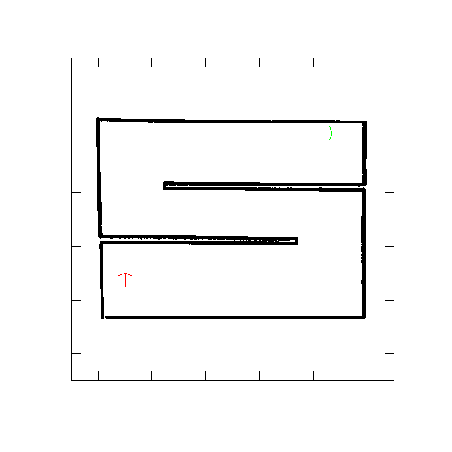
\includegraphics[scale=0.64]{./figures/slides/ch4/corridor}}%
    \gplfronttext
  \end{picture}%
\endgroup

  %\caption{\small Ο χάρτης του περιβάλλοντος CORRIDOR, $\bm{M}_C$, και δύο στάσεις
           %μέσα σε αυτόν, $\bm{p}_a(11.56, 12.2, 0.0)$, και
           %$\bm{p}_b(4.56, 10.2, 0.0)$}
  %\label{fig:map_corridor}
%\end{figure}



Στο σχήμα \ref{fig:map_corridor} παρουσιάζεται ο χάρτης ενός απλού, δομημένου,
μη σύνθετο περιβάλλον που ονομάζεται CORRIDOR, $\bm{M}_C$, στο οποίο πραγματοποιήσαμε μια
αριθμό προσομοιώσεων με ένα ρομπότ εξοπλισμένο με έναν πανοραμικό αισθητήρα LIDAR 2D.
Προκειμένου να εξετάσουμε τον τρόπο με τον οποίο η έξοδος μιας μεθόδου ICP επηρεάζεται από την
τροποποίηση των παραμέτρων της, επιλέξαμε την PLICP \cite{plicp}--την πιο ισχυρή
και με τις καλύτερες επιδόσεις παραλλαγή των μεθόδων αντιστοίχισης σάρωσης με βάση την ICP σε
ρομποτικής--για να πραγματοποιήσει τον εντοπισμό του ρομπότ. Μια προεπιλεγμένη παράμετρος
διαμόρφωση χρησιμεύει ως βάση από την οποία τροποποιούνται $8$ βασικές παράμετροι
μία φορά και στη συνέχεια τίθενται στην προεπιλεγμένη τιμή τους. Προκειμένου να ερευνηθεί η λύση της
τοπίο, εκτελέσαμε τον παγκόσμιο εντοπισμό υπό την προαναφερθείσα
καθεστώς αντιστοίχισης σάρωσης-προς-χάρτη-σάρωσης, για τις πόζες του ρομπότ $\bm{p}_a$ και $\bm{p}_b$,
και δύο διαφορετικά επίπεδα θορύβου, με σταθερό αριθμό σταθερών θέσεων
υποθέσεων, για $10$ φορές, καθιστώντας $N_S = 2 \times 2 \times 14 \times 10 = 560$
προσομοιώσεις.  Η τοποθέτηση των θέσεων διατηρήθηκε σταθερή, ώστε να είναι δυνατή η εκτέλεση
άμεσες συγκρίσεις- δόθηκε προσοχή ώστε το σύνολο του μη κατειλημμένου χώρου
γέμισε με υποθέσεις, και ως εκ τούτου το PLICP δεν λιμοκτονούσε για αντιστοιχίες. Πίνακας
\ref{tbl:csm_diff_params} απεικονίζει τις παραμέτρους υπό τροποποίηση και τις
συνολικό σφάλμα πόζας για κάθε λύση που βρέθηκε.  Το σφάλμα πόζας σχετικά με την πραγματική πόζα
$\bm{p}(x,y,\theta)$ και τη λύση $\bm{\hat{p}}(\hat{x}, \hat{y},
\hat{\theta})$ στο πρόβλημα του παγκόσμιου εντοπισμού για την εν λόγω στάση ανάπαυσης είναι
συμβολίζεται με $e(\bm{p}) = \big((x-\hat{x})^2 + (y-\hat{y})^2 + (\theta -
\hat{\theta})^2\big)^{1/2}$. Η εξαιρετική συμπεριφορά της PLICP--πέραν της
βιβλιογραφία--και η καλή συμπεριφορά του προεπιλεγμένου συνόλου παραμέτρων έχουν
προσδιορίστηκαν ως τέτοιες μετά από εκτεταμένες δοκιμές κατά τη διάρκεια της έρευνας πάνω από tandem
συνδυασμούς φίλτρων σωματιδίων με αντιστοίχιση σάρωσης-σε-χάρτη-σάρωσης
\cite{pose_selection_and_feedback_methods}. Λεπτοµέρειες σχετικά µε τη σηµασία και τη χρήση των
κάθε δηλωμένης και τροποποιημένης παραμέτρου μπορεί να βρεθεί στα \cite{csm_manual1} και
\cite{csm_manual2}.


\begin{table*}\hspace{-1.5cm}
\begin{tabular}{lll|rrr|rr}
  Solution error $e$ regarding robot pose $\bm{p}_{*}$    &  &      & \multicolumn{2}{c}{$e(\bm{p}_a)$} &  & \multicolumn{2}{c}{$e(\bm{p}_b)$} \\ \hline
  Sensor noise $\mathcal{N}(0,\sigma)$, $\sigma$:             & &        & $0.0$                 & $0.01$          &  & $0.0$            & $0.01$         \\ \hline
  Default parameter set               &         &           & $0.006579$        & $0.005601$        &  & $0.036817$         & $0.037745$       \\ \hline
  Parameter modified                  & value   & default   &                   &                   &  &                    &                             \\ \hline
  \texttt{use\_corr\_tricks}          & true    & false     & $0.006579$        & $0.006401$        &  & $0.036817$         & $0.037744$       \\
  \texttt{restart}                    & true    & false     & $0.006579$        & $0.007433$        &  & $0.036818$         & $0.037786$       \\
  \texttt{clustering\_threshold}      & $1.025$ & $0.025$   & $0.006579$        & $0.006051$        &  & $0.036818$         & $0.038122$       \\
  \texttt{do\_alpha\_test}            & false   & true      & $0.006579$        & $0.006972$        &  & $0.036817$         & $0.038493$       \\
  \texttt{orientation\_neighbourhood} & $2$     & $20$      & $0.006579$        & $0.006628$        &  & $0.036818$         & $0.037225$       \\
                                      & $200$   &           & $15.425727$       & $15.425727$       &  & $9.915300$         & $9.915300$         \\
  \texttt{outliers\_maxPerc}          & $0.9$   & $1.0$     & $0.004319$        & $0.006053$        &  & $0.035770$         & $0.035864$       \\
                                      & $0.8$   &           & $0.004486$        & $0.005135$        &  & $0.035900$         & $0.038418$       \\
                                      & $0.7$   &           & $4.709158$        & $0.004731$        &  & $10.298579$        & $0.037788$       \\
  \texttt{outliers\_adaptive\_order}  & $0.9$   & $1.0$     & $0.004472$        & $0.004722$        &  & $0.035586$         & $0.036388$       \\
                                      & $0.8$   &           & $0.004359$        & $0.005790$        &  & $0.036678$         & $0.036897$       \\
                                      & $0.7$   &           & $0.004272$        & $0.004062$        &  & $2.922564$         & $4.498574$       \\
  \texttt{outliers\_remove\_doubles}  & true    & false     & $0.006227$        & $0.006404$        &  & $0.036268$         & $0.036732$       \\
\bottomrule
\end{tabular}
\caption{\small Το σφάλμα πόζας $e(\bm{p})$ για την καλύτερη αντιστοιχία που βρέθηκε από το PLICP στο
         το περιβάλλον CORRIDOR (εικ. \ref{fig:map_corridor}) σε $N_S$
         προσομοιώσεις για ένα προεπιλεγμένο σύνολο παραμέτρων και για ποικίλες τιμές του πυρήνα
         παραμέτρων, και δύο επίπεδα θορύβου του αισθητήρα, ο οποίος υποτίθεται ότι είναι
         κανονικά κατανεμημένος με τυπική απόκλιση $\sigma$ [m]. Η μονάδα του
         μέτρησης του σφάλματος πόζας είναι $(\text{m}^2+\text{rad}^2)^{1/2}$}
\label{tbl:csm_diff_params}
\end{table*}


Ας ξεκινήσουμε την ανάλυση της άστατης συμπεριφοράς του PLICP εστιάζοντας στην
αποτελέσματα όταν ο θόρυβος του αισθητήρα απουσιάζει. Για αυτές τις δύο συγκεκριμένες στάσεις, σε αυτό το
συγκεκριμένο περιβάλλον, η τροποποίηση των παραμέτρων που σχετίζονται με τη χρήση των ενισχυμένων
μεθόδων εύρεσης αντιστοιχιών (\texttt{use\_corr\_tricks}), την επανεκκίνηση
όταν μια λύση υπερβαίνει ένα κατώφλι (\texttt{restart}), ομαδοποίηση των σημείων στο
(\texttt{clustering\_threshold}), δοκιμή μιας λύσης ενώ
λαμβάνοντας υπόψη τον προσανατολισμό της κανονικής της επιφάνειας των σαρώσεων
(\texttt{do\_alpha\_test}), και τον αριθμό των γειτονικών ακτίνων που χρησιμοποιούνται για να
την εκτίμηση του προσανατολισμού
(\texttt{orientation\_neighbourhood} $=2-20$)--- η τροποποίηση αυτών φαίνεται να μην έχει καμία
επίδραση στη λύση για κάθε δοκιμασμένη πόζα ρομπότ. Εάν εξετάσουμε τη θέση
σφάλμα σε σχέση με αυτές τις παραμέτρους όταν υπάρχει θόρυβος του αισθητήρα, παρατηρούμε
ότι η τροποποίηση μιας παραμέτρου μπορεί να έχει θετικό αντίκτυπο στη λύση για
μια πόζα, αλλά αρνητική για μια άλλη (π.χ. \texttt{use\_corr\_tricks},
\texttt{clustering\_threshold}). Επιπλέον, η λειτουργικότητα της οποίας ο σκοπός είναι να
να βελτιώσει την απόδοση της μεθόδου δεν οδηγεί πάντα στο επιθυμητό αποτέλεσμα
(π.χ. \texttt{use\_corr\_tricks}, \texttt{restart}). Η θετική τροποποίηση
άλλων παραμέτρων (π.χ. \texttt{outliers\_remove\_doubles}) παράγει
συνεπή αποτελέσματα σε όλα τα επίπεδα θορύβου των αισθητήρων για μια πόζα ($\bm{p}_b$),
ασυνεπή για άλλα ($\bm{p}_a$), ή συνολικά καταστροφικά λανθασμένα
(\texttt{προσανατολισμός\_γειτονιά} $=200$).





Η υψηλότερη ευαισθησία της PLICP, ωστόσο, παρουσιάζεται όσον αφορά
παραμέτρους που σχετίζονται με το φιλτράρισμα των ακραίων αντιστοιχιών, οι οποίες συμβολίζονται με το
πρόθεμα \texttt{outliers\_}. Η τιμή $1.0-$\texttt{outliers\_maxPerc}
καθορίζει το ποσοστό των αντιστοιχιών με το μεγαλύτερο σφάλμα που πρέπει να
απορρίπτονται, ενώ η τιμή \texttt{outliers\_adaptive\_order} καθορίζει το
κατώτερο ποσοστό των αντιστοιχιών (ανάλογα με το σφάλμα τους) για το οποίο μια
εκτελείται προσαρμοστικός αλγόριθμος για την απόρριψη αντιστοιχιών. Όσον αφορά το
πρώτο, αυτό που παρατηρούμε και για τις δύο στάσεις ρομπότ είναι ότι η απόρριψη των κορυφαίων $30\%$
των πιο λανθασμένων αντιστοιχιών οδηγεί σε καταστροφική αποτυχία ελλείψει
θορύβου των αισθητήρων, αλλά ακριβή συμπεριφορά σε περίπτωση διαταραχών. Όσον αφορά
άλλες τιμές, δεν παρατηρείται συνεπής συμπεριφορά, αν και όλες οδηγούν σε
σωστή σύγκλιση. Όσον αφορά το τελευταίο, η ασυνέπεια μεταξύ
μεταξύ των αποτελεσμάτων προκύπτει σε επίπεδο διαφορετικών στάσεων- η ρύθμιση αυτής της παραμέτρου σε
$70\%$ παρουσιάζει αυξημένη ακρίβεια για $\bm{p}_a$, αλλά καταστροφική αποτυχία σε
σύγκλισης για το $\bm{p}_b$.

Η παραπάνω ανάλυση πραγματοποιήθηκε προκειμένου να καταδειχθούν οι αμηχανίες
στις οποίες μπορεί να βρεθεί μια υγιής μέθοδος όταν βασίζεται σε συντονισμό λεπτών
εσωτερικών παραμέτρων. Ακόμη και αν όλες οι τιμές που δοκιμάστηκαν είχαν ως αποτέλεσμα τη σωστή σύγκλιση,
το ζήτημα της (μη) συνέπειας σε διαφορετικά επίπεδα θορύβου του αισθητήρα και διαφορετικές
πόζες εντός του ίδιου χάρτη θα παρέμενε, μαζί με αυτό της ασυνέπειας
της διαίσθησης σχετικά με την επίδρασή τους. Ως εκ τούτου, καταλήγουμε στο συμπέρασμα ότι το πλεονέκτημα της
προσαρμογής των παραμέτρων σε συγκεκριμένες περιστάσεις δεν είναι χωρίς τα πλεονεκτήματά του, αλλά
τις παρενέργειές του. Στη συνέχεια, και ανακεφαλαιώνοντας, θα ήταν
αξιέπαινη για την έρευνα να επικεντρωθεί σε μεθόδους εκτίμησης της πόζας που δεν χρειάζονται
την καθιέρωση αντιστοιχιών και τη ρύθμιση των παραμέτρων για διαφορετικές πόζες
και περιβάλλοντα.



